\documentclass[amssymb,twocolumn,aps]{revtex4}

% allows special characters (including æøå)
\usepackage[utf8]{inputenc}
%\usepackage [norsk]{babel} %if you write norwegian
\usepackage[english]{babel}  %if you write english

\usepackage{physics,amssymb}  % mathematical symbols (physics imports amsmath)
\usepackage{graphicx}         % include graphics such as plots
\usepackage[table]{xcolor}
\usepackage{xcolor}           % set colors
\usepackage{hyperref}         % automagic cross-referencing 
\usepackage{float}			  % force placement of tables and figures
\usepackage{comment}
%\usepackage[authoryear]{natbib}
\usepackage{algorithm}
\usepackage{amsthm}
\usepackage{algpseudocode}



\newtheorem{prop}{Proposition}[section]

\begin{document}

\title{Report Template \\
    \normalsize FYS-STK3155 - Project X}
\date{\today}               
\author{
    Anton Nicolay Torgersen 
}
\affiliation{University of Oslo}


\newpage


%Abstract: accurate and informative? Total number of possible points: 5

    \begin{abstract}
A study of various regression methods, including OLS, Ridge and LASSO and how they fit Runge's function. 
We review the theory and implementation of these methods and see how they compare on this function.
At the end, we discuss some resampling techniques on the simpler OLS-method to understand the bias-variance trade-off.
\end{abstract}


    \maketitle
    \thispagestyle{empty} % Removes page number from the title page

    


% Introduction: status of problem and the major objectives. Total number of possible points: 10
\section{Introduction}

The fundamental problem in machine learning and statistics is to find meaningful patterns in data using models that make accurate predictions on unseen data.
This is a difficult task, as a complex function might fit the training data perfectly, but fail spectacularly when facing new instances, a phenomenon known as overfitting.
On the other hand a model that is too simple may fail to extract the patterns in the data and thus underfit the data.
Therefore understanding of the bias-variance tradeoff on simpler models before the more complex ones is paramount to develop robust and generalizable models.

Therefore, this paper will study the bias-variance tradeoff through the lens of regression models, that increase in complexity.
We start with the simplest model, Ordinary Least Squares (OLS), where we have a fully analytical solution for the best fit parameters.
Then we move on to Ridge regression, which is a regularized version of OLS, where we first introduce the tuning of a penalization parameter $\lambda$ to find a good balance between bias and variance.
Finally we end with LASSO regression, which is another regularized version of OLS, but with a different penalization term.

This analysis will closely follow the lecture notes from FYS-STK3155 \cite{compfys} and the book "The Elements of Statistical Learning" by Hastie, Tibshirani and Friedman \cite{hastie}.
We will review the theory of the three regression methods and apply the methods to a one-dimensional problem, fitting a polynomial model to Runge's function, $f(x)=1/(1+25x^2)$.
This function is notoriously difficult for high-degree polynomial interpolation and will therefore be a good demonstration of the pitfalls of overfitting and the benefits of regularized techniques like Ridge and LASSO.
Together these three models will create a better understanding of the dynamics between bias and variance, how the dynamic shifts with model complexity and methods.
The result is a better intuition for tuning models, when is the model inching towards the true function $y$ and when is it stuck in a well. 


\begin{comment}
When you write the introduction you should focus on the following aspects:
\begin{itemize}
    \item Motivate the reader, the first part of the introduction gives always a motivation and tries to give the overarching ideas. Citing some central ideas or problems in the literature is a good idea here. \cite{compfys}\cite{eigenvalue}\cite{hein, hastie}
    \item What you have done, with a focus on choice of problem and method, and why these were chosen.
    \item The structure of the report, how it is organized. List the sections, and very briefly describe what is in them and how they fit together.
\end{itemize}
\end{comment}

\section{Methods}\label{section:methods}
We will be assuming that the reader has some familiarity with linear algebra and multivariable calculus.
For a more in-depth review of the methods and algorithms, including the motivation for using them and their applicability to the problem, please refer to the lecture notes \cite{compfys} and the book "The Elements of Statistical Learning" by Hastie, Tibshirani and Friedman \cite{hastie}.
For the scoring measures Mean Squared Error (MSE) and R2, please refer to \cite{scoring1} section 2.2.1 and 3.1.3 for information or see the implementation in the code.

\subsection{Regression Methods}
We will be studying three regression methods: Ordinary Least Squares (OLS), Ridge regression and LASSO regression.
All three methods are used to fit a polynomial model to the data, but they differ in how they estimate the model parameters and how they handle overfitting.

The problem we are tyring to solve is to find a polynomial function $\tilde{y}(x)$ that approximates the true function $y(x)$, given a set of data points $(x_i, y_i)$, where $i=1,2,...,n$.

\subsubsection{Ordinary Least Squares (OLS)}
The simplest of the three methods, it is defined by minimizing the sum of the squared differences between the observed values $y_i$ and the predicted values $\tilde{y}_i$.

$$C(\theta) = \frac{1}{n} \sum_{i=1}^{n} (y_i - \tilde{y}_i)^2$$

where $\tilde{y} = X\theta$, $X$ is the design matrix, $\theta$ is the vector of model parameters and $y$ is the vector of observed values.

Taking the derivative with reagrds to $\theta$ equal to $0$ gives rise to an analytical solution with no relance on $\theta$:
\begin{equation}
  \theta = (X^TX)^{-1}X^Ty  
\end{equation}
This solution is valid as long as $X^TX$ is invertible, which is the case when the columns of $X$ are linearly independent, and if they are not one can just shift the diagonal slightly.

We also have a gradient descent solution to this problem by taking the derivative of the cost function with reagrds to $\theta$ and updating $\theta$ iteratively.
\begin{align}
\nabla_{\theta_n} &= \frac{1}{n}2X^T(X\theta_n + y) \\
\theta_{n+1} &= \theta_n - \eta \nabla_{\theta_n}
\end{align}
where $\eta$ is the learning rate that controls the step size in the parameter space.

\subsubsection{Ridge Regression}
This is a regularized version of OLS, where we add a penalization term to the cost function to prevent overfitting.
$$
    C(\theta, \lambda) = \frac{1}{n} \sum_{i=1}^{n} (y_i - \tilde{y}_i)^2 + \lambda \sum_{j=1}^{p} \theta_j^2
$$

where $\lambda$ is the regularization parameter that controls the strength of the penalization and $p$ is the number of model parameters, in our case the degree of the polynomial.
The analytical solution is given by:
\begin{equation}
\theta = (X^TX + \lambda I)^{-1}X^Ty
\end{equation}
where $I$ is the identity matrix.

We also have a gradient descent solution to this problem by taking the derivative of the cost function with reagrds to $\theta$ and updating $\theta$ iteratively \cite{compfys}(week 36).
\begin{align*}
\nabla_{\theta_n} &= \frac{1}{n}2X^T(X\theta_n - y) + 2\lambda \theta_n \\
\theta_{n+1} &= \theta_n - \eta \nabla_{\theta_n}
\end{align*}

\subsubsection{LASSO Regression}
Lasso is defined by minimizing the following cost function:
$$
C(\theta, \lambda)=\frac{1}{n}\sum^n_{i=1}(y_i- \tilde{y_i})^2+\lambda \sum_{j=1}^p\vert \theta_j\vert
,$$
which is a also regularized version of OLS except using the norm on the parameter vector.
The penalty term has the effect of driving some parameter estimates $\theta_j$ to exactly zero, which performs feature selection and results in a simpler, sparser model.

Because the cost function is not differentiable an analytical solution does not exist.
The problem must be solved iteratively using the two steps one from solving the term without the regularization just as with OLS another for the regularization term.
Where we take a soft cap on the parameters based on a regularization value\ref{alg:lasso_ista}.

\begin{algorithm}
\caption{LASSO Regression using Gradient Descent }
\label{alg:lasso_ista}
\begin{algorithmic}[1]
\State \textbf{Initialize:} $\theta_0$, learning rate $\eta$, regularization parameter $\lambda$
\State \textbf{Define:} $\alpha \leftarrow \eta \lambda$
\For {$t = 0$ to $N_{\text{iters}}-1$}
    \State $\nabla_{\text{OLS}} \leftarrow \frac{2}{n}X^T(X\theta_t - y)$
    \State $\mathbf{z} \leftarrow \theta_t - \eta \cdot \nabla_{\text{OLS}}$
    \State $\theta_{t+1}^j \leftarrow \text{sgn}(\mathbf{z}_j) \cdot \max(0, |\mathbf{z}_j| - \alpha) \quad \forall j \in \{1, \dots, p\}$
\EndFor
\State \textbf{Return:} $\theta_{N_{\text{iters}}}$
\end{algorithmic}
\end{algorithm}

For more on these three methods see \cite{compfys} and \cite{hastie}.
\subsection{Gradient Descent}

\subsubsection{Changing learning rate algorithms}
\textbf{Momentum}

It's a technique that helps accelerate gradient descent by adding a fraction of the previous update to the current update. This helps to smooth out the updates and can lead to faster convergence. The update rule becomes:
\begin{align*}
v_{t+1} &= \beta v_t + (1 - \beta) \nabla_{\theta} J(\theta_t) \\
\theta_{t+1} &= \theta_t - \eta v_{t+1}
\end{align*}
where $v_t$ is the velocity (the exponentially weighted average of the gradients), $\beta$ is the momentum term (usually set to 0.9), and $\eta$ is the learning rate.
\\

\textbf{Adagrad}

This technique adapts the learning rate for each parameter based on the historical sum of squared gradients. This means that parameters with larger gradients will have smaller learning rates, and vice versa. The update rule is:
\begin{align*}
\theta_{t+1} &= \theta_t - \frac{\eta}{\sqrt{G_t + \epsilon}} \odot \nabla_{\theta} J(\theta_t)
\end{align*}
where $G_t$ is the diagonal matrix of the sum of squared gradients up to time $t$, and $\epsilon$ is a small constant added for numerical stability.
\\

\textbf{RMSprop}

This technique is similar to ADAgrad but uses a moving average of the squared gradients instead of the cumulative sum. This helps to prevent the learning rate from becoming too small. The update rule is:
\begin{align*}
\theta_{t+1} &= \theta_t - \frac{\eta}{\sqrt{E_t + \epsilon}} \odot \nabla_{\theta} J(\theta_t)
\end{align*}
where $E_t$ is the moving average of the squared gradients.
\\

\textbf{Adam}

Adam (Adaptive Moment Estimation) combines the ideas of momentum and RMSprop. It maintains both a moving average of the gradients and a moving average of the squared gradients. The update rule is:
\begin{align*}
m_{t+1} &= \beta_1 m_t + (1 - \beta_1) \nabla_{\theta} J(\theta_t) \\
v_{t+1} &= \beta_2 v_t + (1 - \beta_2) (\nabla_{\theta} J(\theta_t))^2 \\
\theta_{t+1} &= \theta_t - \frac{\eta}{\sqrt{v_{t+1}}} \odot m_{t+1}
\end{align*}
where $m_t$ is the moving average of the gradients, $v_t$ is the moving average of the squared gradients, $\beta_1$ is usually set to 0.9, and $\beta_2$ is usually set to 0.999.

\subsubsection{Stochastic Gradient Descent}
Stochastic Gradient Descent (SGD) is a variant of gradient descent where the model is updated using only a single training example (or a small batch) at each iteration, rather than the entire dataset. This can lead to faster convergence, especially for large datasets, and can help to escape local minima.

The update rule for SGD is similar to that of standard gradient descent:
\begin{align*}
\theta_{t+1} &= \theta_t - \eta \nabla_{\theta} J(\theta_t; x_i, y_i)
\end{align*}
where $(x_i, y_i)$ is a single training example.

SGD introduces noise into the optimization process, which can be beneficial for escaping local minima but may also lead to instability in the convergence process. To mitigate this, techniques such as learning rate schedules and mini-batch training are often employed.

\subsection{Sampling methods}

Show that you can rewrite this in terms of a term which contains the variance of the model itself
(the so-called variance term), a term which measures the deviation from the true data and the mean
value of the model (the bias term) and finally the variance of the noise.

\begin{prop}
For a model $\tilde{y}$ that approximates the true function $y$, the expected mean squared error can be decomposed into three components: the variance of the model, the squared bias of the model, and the variance of the noise. Mathematically, this is expressed as:
$$\mathbb{E}[(y-\tilde{y})^2] = \mathrm{bias}[\tilde{y}]^2 + \mathrm{var}[\tilde{y}] + \sigma^2$$
where $\mathrm{bias}[\tilde{y}] = \mathbb{E}[\tilde{y}] - y$, $\mathrm{var}[\tilde{y}] = \mathbb{E}[(\tilde{y} - \mathbb{E}[\tilde{y}])^2]$, and $\sigma^2$ is the variance of the noise in the data.
\end{prop}

\begin{proof}

First, write out what the terms are for the expectation value of $\mathbb{E}[(y-\tilde{y})^2]$:

\begin{align*}
\mathbb{E}[(y-\tilde{y})^2 ]&= \mathbb{E}[(y-\tilde{y}) (y-\tilde{y}) ] \\
&= \mathbb{E}[(y^2-\tilde{y} y -y \tilde{y} +\tilde{y}^2)] \\
&= \mathbb{E}[y^2] - 2 \mathbb{E}[\tilde{y} y] +\mathbb{E}[\tilde{y}^2] \\
\end{align*}

Looking into the function $\mathbb{E}[\tilde{y}^2]$ and using $\mathrm{var}[\tilde{y}] = \mathbb{E}[y^2] - \mu_y^2$ we see that this can be written as 
$$
\mathbb{E}[\tilde{y}^2] = \mathrm{var}[\tilde{y}] + \mathbb{E}[\tilde{y}]^2.
$$

Secondly looking closer at $\mathbb{E}[y^2]$ and writing the function $y$ as $f + \varepsilon$, where we assuming $f$ to be non stochastic and $\varepsilon \sim N(0, \sigma^2)$, we get:

$$
\mathbb{E}[(f+\varepsilon)^2] = \mathbb{E}[f^2] + 2 \mathbb{E}[f]\mathbb{E}[\varepsilon] + \mathbb{E}[\varepsilon^2] = \mathbb{E}[f^2] + \sigma^2 = f^2 + \sigma^2
$$

Lastly the term $\mathbb{E}[\tilde{y} y]$, becomes the following since $\tilde{y}$ and $\varepsilon$ are independent and we can distribute the expectation operation.

$$
\mathbb{E}[\tilde{y} (f + \varepsilon)] = \mathbb{E}[\tilde{y} f] + \mathbb{E}[\tilde{y} \varepsilon] = f \mathbb{E}[\tilde{y}] + 0
$$

Taking everything together we get:

\begin{align*}
&=\mathbb{E}[y^2] - 2 \mathbb{E}[\tilde{y} y] +\mathbb{E}[\tilde{y}^2] \\
&= f^2 + \sigma^2 - 2 f \mathbb{E}[\tilde{y}] +\mathrm{var}[\tilde{y}] + \mathbb{E}[\tilde{y}]^2 \\
&= f^2 - 2 f \mathbb{E}[\tilde{y}] + \mathbb{E}[\tilde{y}]^2 + \mathrm{var}[\tilde{y}] + \sigma^2 \\
&= \mathbb{E}[ (f - \mathbb{E}[\tilde{y}])^2] + \mathrm{var}[\tilde{y}] + \sigma^2 \\
&= \mathrm{bias}[\tilde{y}]  + \mathrm{var}[\tilde{y}] + \sigma^2 \
\end{align*}

Where we have approximated $f$ with $y$, in the last step in order to evaluate it as f is unknown
\end{proof}


\subsubsection{Bootstrap}


\subsubsection{Cross Validation}


part g, write about the implementation of the bootstrap method as a resampling technique on the OLS method.
part h, write about the implementation of the k-fold cross-validation algorithm as a resampling technique on the OLS, Ridge and LASSO methods.

\begin{comment}
\begin{itemize}
    \item Describe the methods and algorithms, including the motivation for using them and their applicability to the problem
    \item Derive central equations when appropriate, the text is the most important part, not the equations.
\end{itemize}
\end{comment}
\subsection{Implementation}
To evaluate the performance of the regression methods and to elucidate the intricacies of the methods and the bias-variance tradeoff we are using Runge's function as a test case.
This is a one-dimensional function

$$
f(x) = \frac{1}{1 + 25x^2},
$$

that is know to be difficult to fit with high-degree polynomials.

We will generate two a data sets of $n$ points, $x_i$, uniformly distributed in the interval $[-1, 1]$, one with and one without noise.
The noisy data set will be generated by adding Gaussian noise $\epsilon_i \sim \mathcal{N}(0, \sigma^2)$ to the function values.



Implementation of the analytical solution of OLS regression using the numpy function pinv {citation???}.
\subsubsection{Regression methods}

perhaps simply a reference to the code for the implementation using numpy.
And a test with the scikit library to see that the implementation is correct for these two.

Maybe some extra for the Lasso implementation?

\subsubsection{Gradient Descent}
part c, write about how we implementation of the gradient descent algorithm for OLS and Ridge regression.
Again squeez it tohether we the above section and reference the code and functions.

\subsubsection*{Changing learning rate}

When we updated our gradient descent function to include momentum we got the following figure \ref{fig:GradMomentum} 


\begin{figure*}[t]
    \centering
    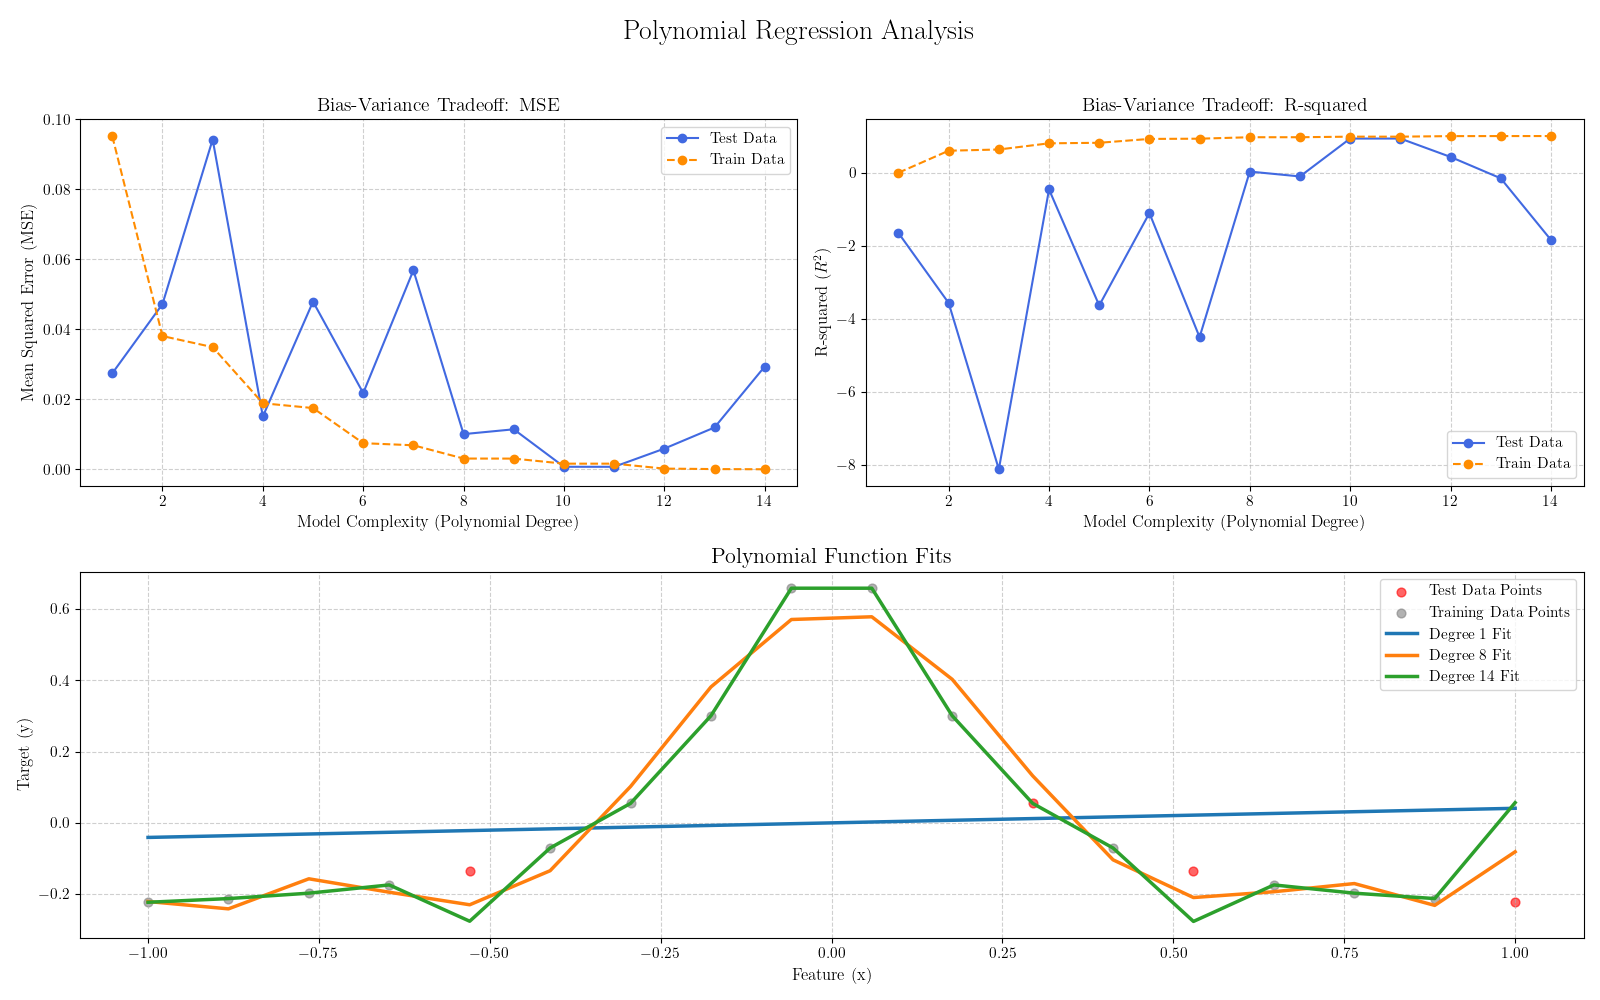
\includegraphics[width=.95 \textwidth]{Figures/Combined_Analysis_OLS.png}
    \caption{OLS and model complexity with N = 18}
    \label{fig:OLS1}
\end{figure*}



part,d implementation of the changing learning rate algorithms: momentum, ADAgrad, RMSprop and Adam.
Follows the implementations from the lecture notes from week 37 \cite{compfys} and is explained in the code.
Function  bla bla bla


\subsubsection*{Stochastic Gradient Descent}
part f, write about the implementation of the stochastic gradient descent algorithm for OLS and Ridge regression.

\subsubsection{Resampling techniques}
part g, write about the implementation of the bootstrap method as a resampling technique on the OLS method.

PROBABLY NOT.part h, write about the implementation of the k-fold cross-validation algorithm as a resampling technique on the OLS, Ridge and LASSO methods.


\begin{comment}
\begin{itemize}
    \item Explain how you implemented the methods and also say something about the structure of your algorithm and present very central parts of your code, not more than 10 lines
    \item You should plug in some calculations to demonstrate your code, such as selected runs used to validate and verify your results. A reader needs to understand that your code reproduces selected benchmarks and reproduces previous results, either numerical and/or well-known closed form expressions.
\end{itemize}
\end{comment}


\subsection{Use of AI tools}
	AI has been used to format and proofread the report and to spot errors in the code.
\begin{itemize}
    \item Describe how AI tools like ChatGPT were used in the production of the code and report.
\end{itemize}




\section{Results and Discussion}\label{section:results}

Description of the function, why it is interesting to study.



Generation of the data set and why and how we scaled it. \textbf{part a)}
We had a set with and without noise in a normal distribution to see how the methods performed on both.
We scaled the data so that the higher polynomials don't take over the cost function making it skewed towards the higher once.
Since most of our analysis will be around a sparse dataset we will be using the noiseless one for the main analysis.
Looking at the figure \ref{fig:OLS1} one can see the function and the datapoints we are trying to fit towards.
This will be the same for all graphs unless otherwise stated.

\textbf{Run through the graphs on the noisey one also and have the comparison as an appendix if it doesn't give any useful information}


Analysis using the methods described in section \ref{section:methods}.

\subsection{Analytical Regression methods}

\subsubsection{Ordinary Least Squares (OLS)}



We first analyzed how OLS works on a small dataset as with more data the variances in training is harder to see. In the figure \ref{fig:OLS1} we see that the data that it trains one becomes better and better the more complex the model becomes as it then has more parameters to model the data on. While the test data becomes much worse when the complexity is close to the number of data points. This implies that the training now fits the points rather than the underlying curve.

\textbf{some thoughts on the R2}


Analyzing how the relationship between datapoints and training at figure\ref{fig:OLSHeat} we see, as we expect, along the borders where there is low training data or low complexity are the worst performing parts on the test data. The yellow spots in the heatmap are capped at 0.1, as these points are prone to explode just as the graph \ref{fig:OLS1} is beginning to do.
A clear case of where the tradeoff between bias and variance goes towards high bias.

\begin{figure}[H]
    \centering
    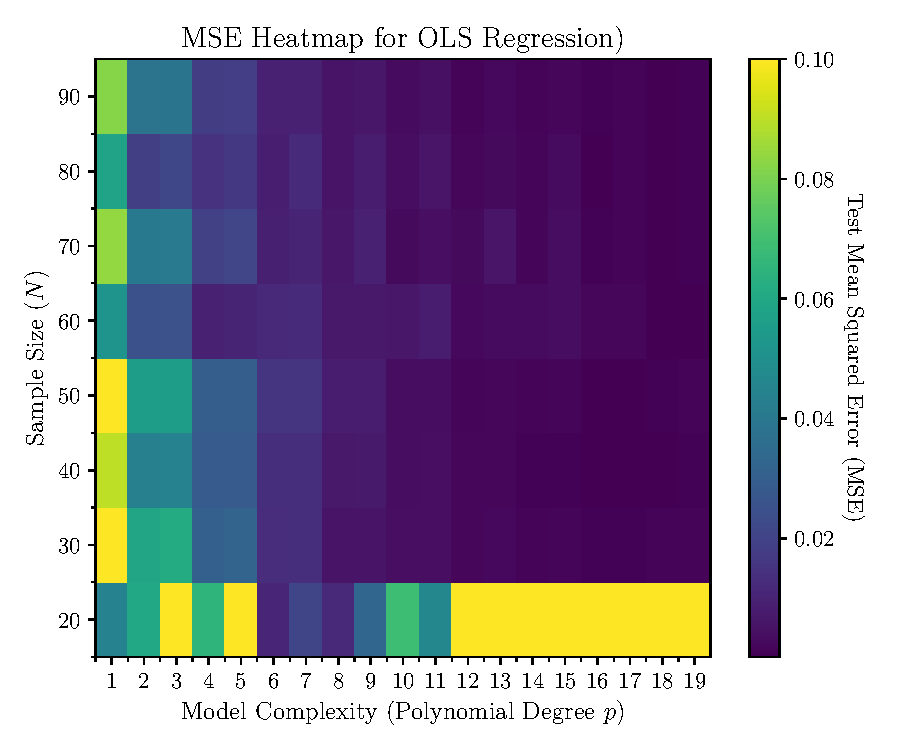
\includegraphics[width=.95 \linewidth]{Figures/OLS_Heatmap.pdf}
    \caption{Data size and Model Complexity}
    \label{fig:OLSHeat}
\end{figure}

\subsubsection{Ridge Regression}
Doing the same training but using Ridge as our method we got some interesting results that elucidates the differences between these models.
Both has there improvements increasing as the complexity increases the differences are in the lows and the highs.
Where the OLS method\ref{fig:OLS1} had a really low value at degree 10, it also begins to diverge a lot at degree 14.
The Ridge method on the other hand stays remarkably consistent here as seen by the training value. 
Implying that the regularization terms take over and keeps the model from fitting the training data to closely. 

\begin{figure}[h]
    \centering
    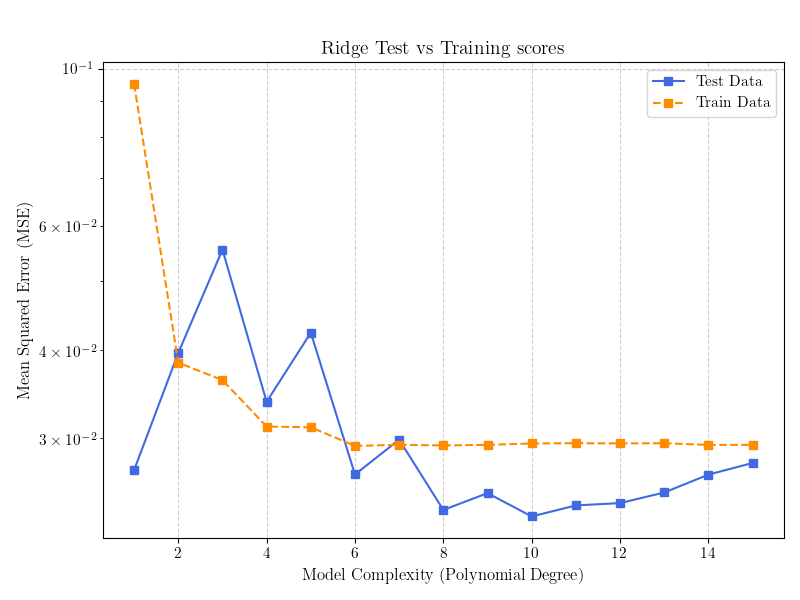
\includegraphics[width=.95 \linewidth]{Figures/MSE_RidgeOnly.png}
    \caption{Ridge and model complexity}
    \label{fig:RidgeMse}
\end{figure}

Now looking closer at the regularization performs with regards to the complexity \ref{fig:RidgeHeat} we get that the regularization step cannot be to high as the model will then fail to learn anything and can struggle a bit at lower values when the model complexity increase with the training data.
The model will fit the data to well before the regularization strikes in, though there are some odd lines in this lower right area.

When we generated an equivalent map as the one above see appendix we get the same results as once can infer from figure \ref{fig:RidgeMse}, lower regularization rates and higher sample sizes gives better models.


\begin{figure}[h]
    \centering
    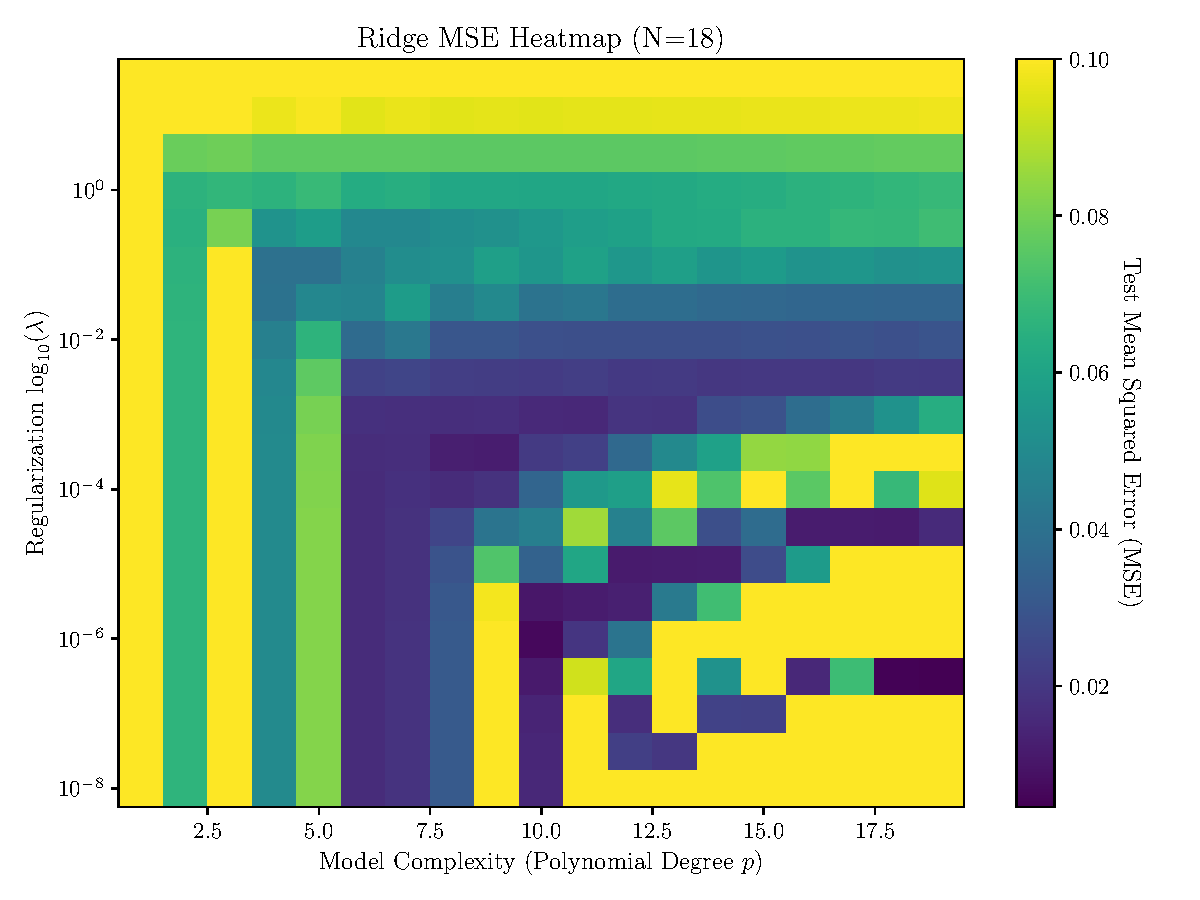
\includegraphics[width=.95 \linewidth]{Figures/Ridge_Degree_Lambda_Heatmap.pdf}
    \caption{Regularization and model complexity}
    \label{fig:RidgeHeat}
\end{figure}

\textit{part b}, important to study the dependence on $\lambda$ the regularization parameter

\subsection{Using Gradient Descent}

\subsubsection{OLS and Ridge with gradient descent}

Doing the calculation based on the gradient solution to the optimization problem, we see that it requires some iterations before one gets close to reaching a sort of minimum on the test set\ref{fig:DescOLSRidge}.
The more complex models also struggle to beat the simplest model in performance, only the polynomial of degree 12 goes below it near the end.
If we had changed the learning rate to be a higher number we would get a faster convergence to the minimum.
But then we will also start to see that it can begin to switch in the other direction and jump as OLS-12 is doing.

We also see that only the simples Ridge model is plateauing and being dominated by the regularization term, suggesting that a higher iteration count or learning rate is necessary.


\begin{figure}[h]
    \centering
    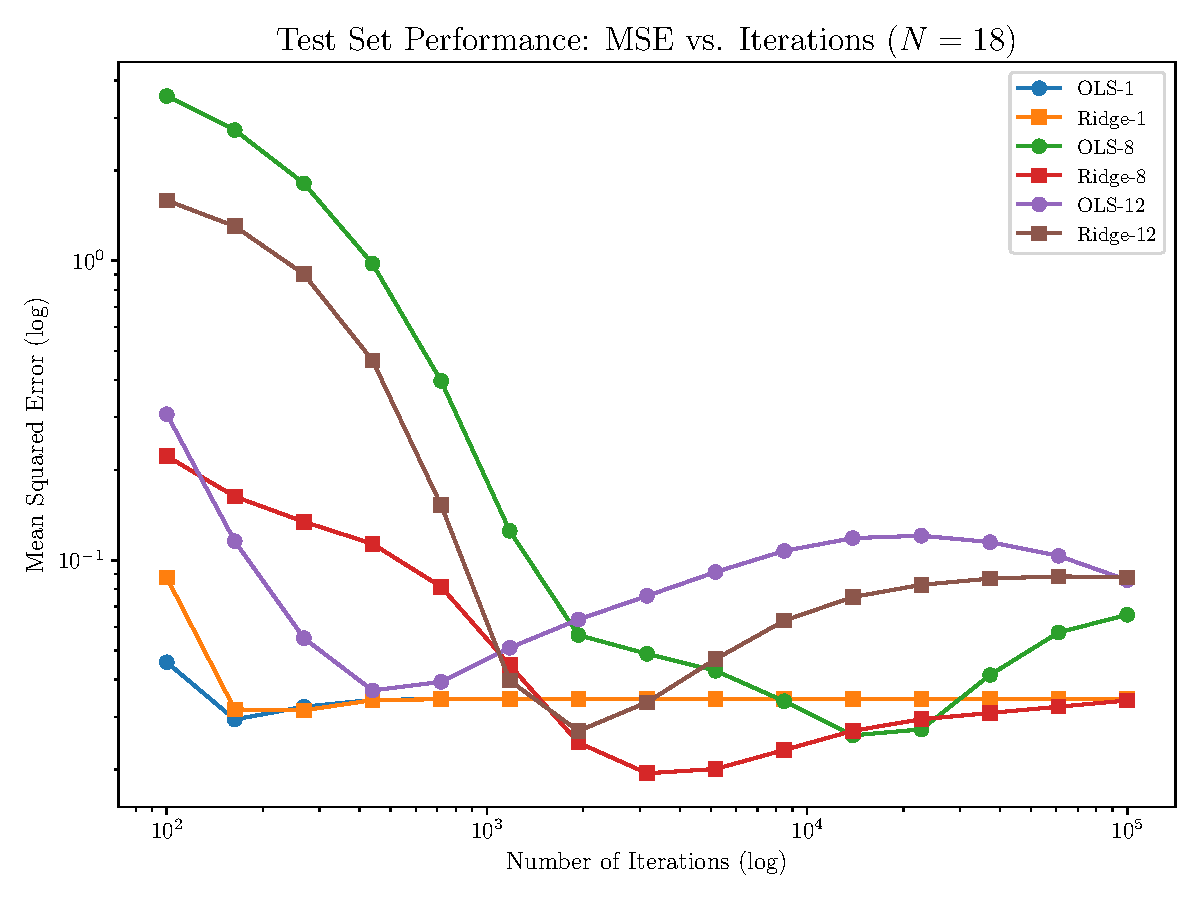
\includegraphics[width=.95 \linewidth]{Figures/Gradient_Comparison_OLS_Ridge_18.pdf}
    \caption{Gradient descent for OLS and Ridge}
    \label{fig:DescOLSRidge}
\end{figure}




\textit{part c},Study the results from the gradient descent algorithm for both OLS and Ridge regression and especially the dependence on the learning rate $\eta$ and the number of iterations. maybe add an other graph of with higher learning rate.



\subsubsection{LASSO Regression}
When we did the same analysis using Lasso regression but with the same parameters and dataset we see in figure \ref{fig:Lasso1} that OLS and Lasso are really similar in how the models improves.


\begin{figure}[h]
    \centering
    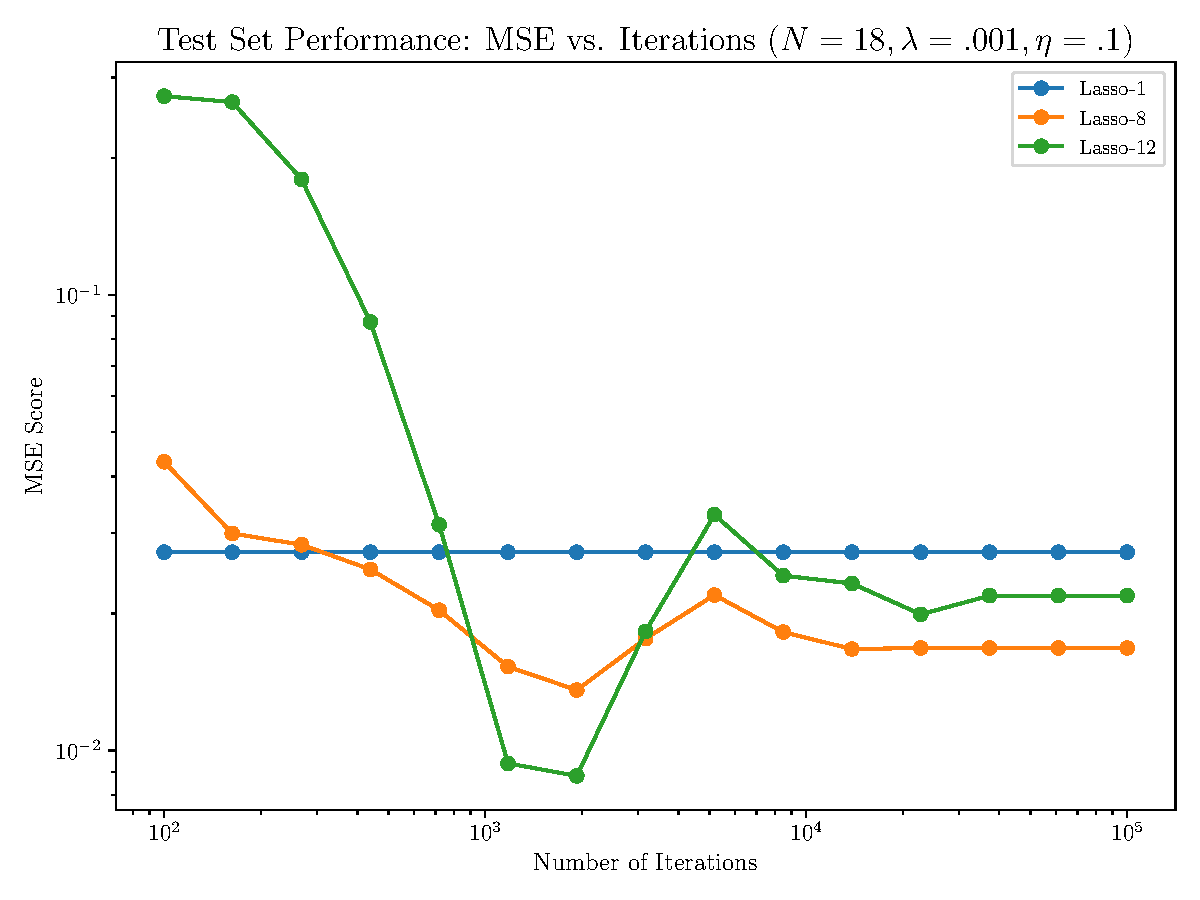
\includegraphics[width=.95 \linewidth]{Figures/Lasso_MSE.pdf}
    \caption{Lasso learning}
    \label{fig:Lasso1}
\end{figure}


part f, study the results from the stochastic gradient descent algorithm for both OLS, Ridge and Lasso regression and especially the dependence on the learning rate $\eta$ and the number of iterations.

\subsection{Learning Rate Algorithms}

For simplicity in implementation we will only be using the OLS and Ridge methods here as they are similar in their gradient descent implementation.
We will use the same dataset as before with 18 points and a learning rate of 0.1 for the normal gradient descent.
Where we will also keep the hyperparameters for the different methods the same throughout the images, to make it easier to compare the methods.

?? include or not \textit{See appendix for analysis on different hyperparameters}

\subsubsection{Momentum}

The first method we tried when changing the learning rate was to implement a momentum term in the gradient descent algorithm.
In our first we saw that the momentum term was to high for seeing the results we wanted as it was visible how it made the model slowed down.
So we lowered it to 0.6 and got the results in figure \ref{fig:GradMomentum}.
We see that the momentum term helps the models to converge faster to a minimum and also helps the more complex models to get a better performance.
When most of the models are beginning to plateau.
\\
\begin{figure}[h]
    \centering
    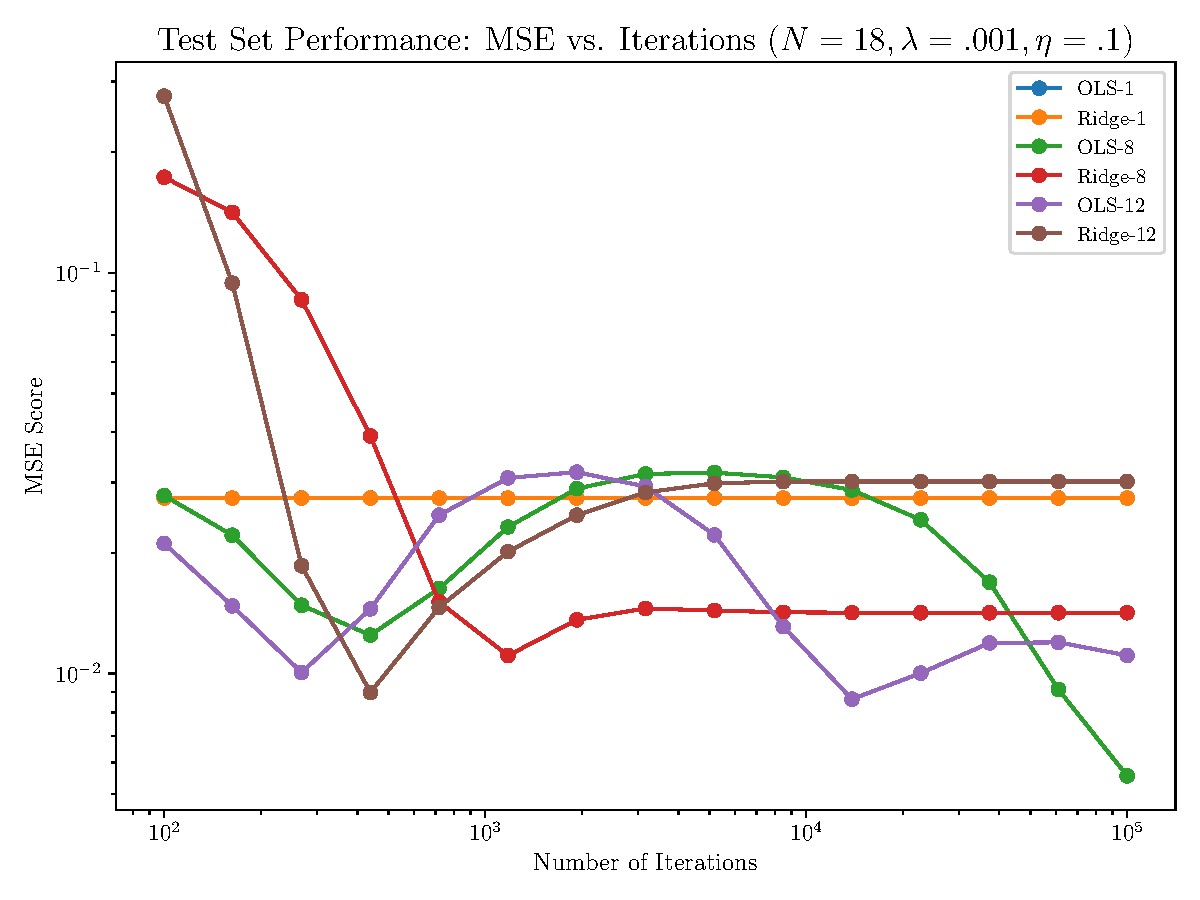
\includegraphics[width=.95 \linewidth]{Figures/OLS_Ridge_Momentum.pdf}
    \caption{Gradient descent with momentum (0.6)}
    \label{fig:GradMomentum}
\end{figure}


\subsubsection{ADAgrad}

Our results from the ADAgrad method are shown in figure\ref{fig:GradADAgrad}.
Here we see that the model converges much slower and seems to struggle at the end to find a position compared to the momentum method or the normal gradient descent.
This is due to the fact that the learningrate starts small and becomes much smaller through ADAgrad.
\\

\begin{figure}[h]
    \centering
    \includegraphics[width=.95 \linewidth]{Figures/OLS_Ridge_ADAgrad.pdf}
    \caption{Gradient descent with ADAgrad (1e-8)}
    \label{fig:GradADAgrad}
\end{figure}


\subsubsection{RMSprop}

When we look at our results are much more volatile as seen in figure \ref{fig:GradRMSprop}.
The simpler models has smaller swings while the more complex models has larger swings with no clear convergence, except for OLS-12. 
This is due to the fact that the learning rate is changing based on the gradient squared and the momentum of this.
Since the learningrate is quite large 0.1 and the dataset is small the model can jump around a lot.
\\

\begin{figure}[h]
    \centering
    \includegraphics[width=.95 \linewidth]{Figures/OLS_Ridge_RMSprop.pdf}
    \caption{Gradient descent with RMSprop (1e-2, 0.9)}
    \label{fig:GradRMSprop}
\end{figure}

\subsubsection{Adam}

Using the Adam method that combines the momentum and RMSprop methods on our dataset.
We see that the figure \ref{fig:GradADAM} has lost much of it's volatility the iterations are less volatile in swings than with the other three methods.
\\

\begin{figure}[h]
    \centering
    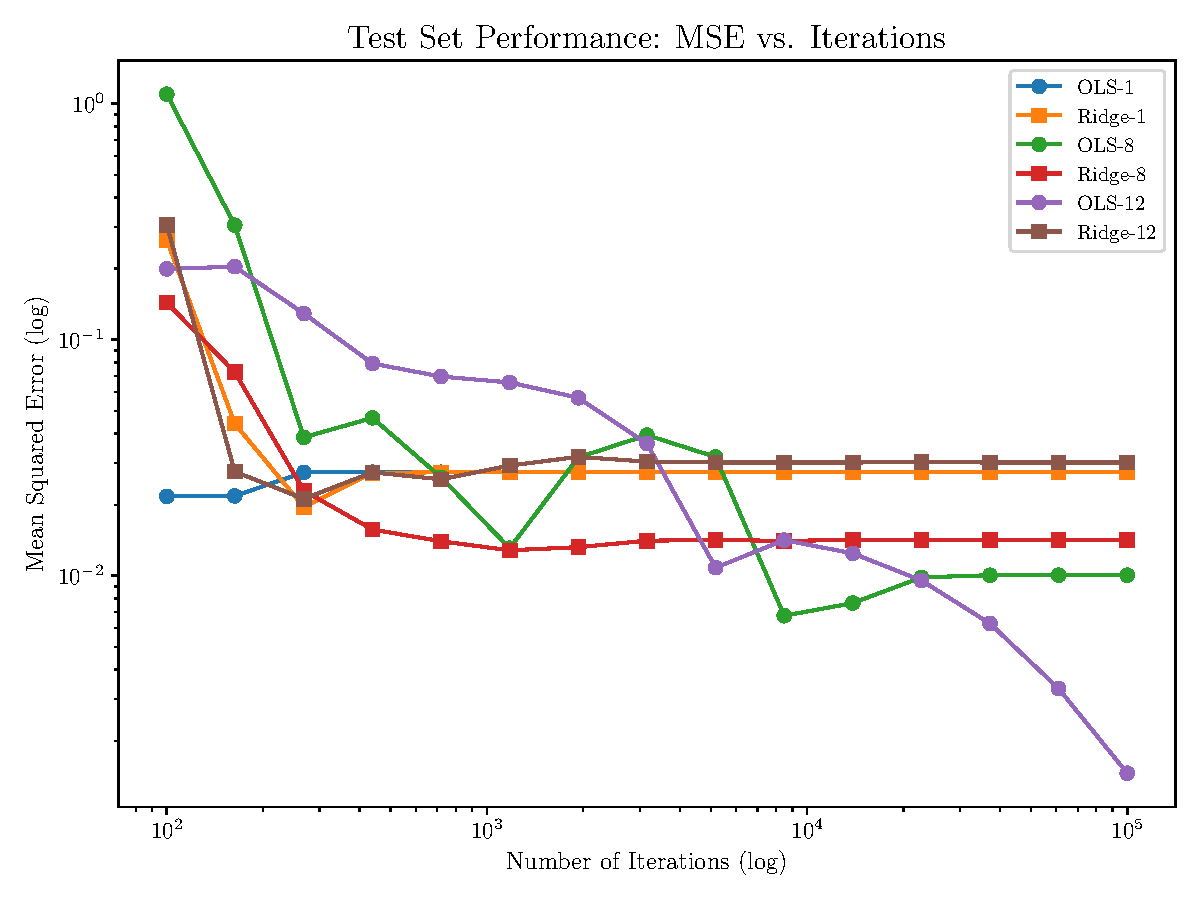
\includegraphics[width=.95 \linewidth]{Figures/OLS_Ridge_ADAM.pdf}
    \caption{Gradient descent with ADAM (1e-2, 0.9)}
    \label{fig:GradADAM}
\end{figure}


\subsection{Stochastic Gradient Descent}
Our results from the stochastic gradient descent method will not be as effiecnt here as we are dealing with a small dataset.
Our batch size is 1/3 of the dataset, so 6 points.
This means that the model will be updated 3 times per epoch.
We see in figure \ref{fig:GradSGD} that the model is much more volatile than the other methods.
This is due to the fact that the model is updated more frequently and with less data.
This means that the model can jump around more and is more prone to overfitting the training data.

The results we got when we decrease the learning rate to 0.01 is that the model becomes less volatile but also converges much slower.
After 100000 iterations it is still not at a decided state except for the linear models.
\\



\begin{figure}[h]
    \centering
    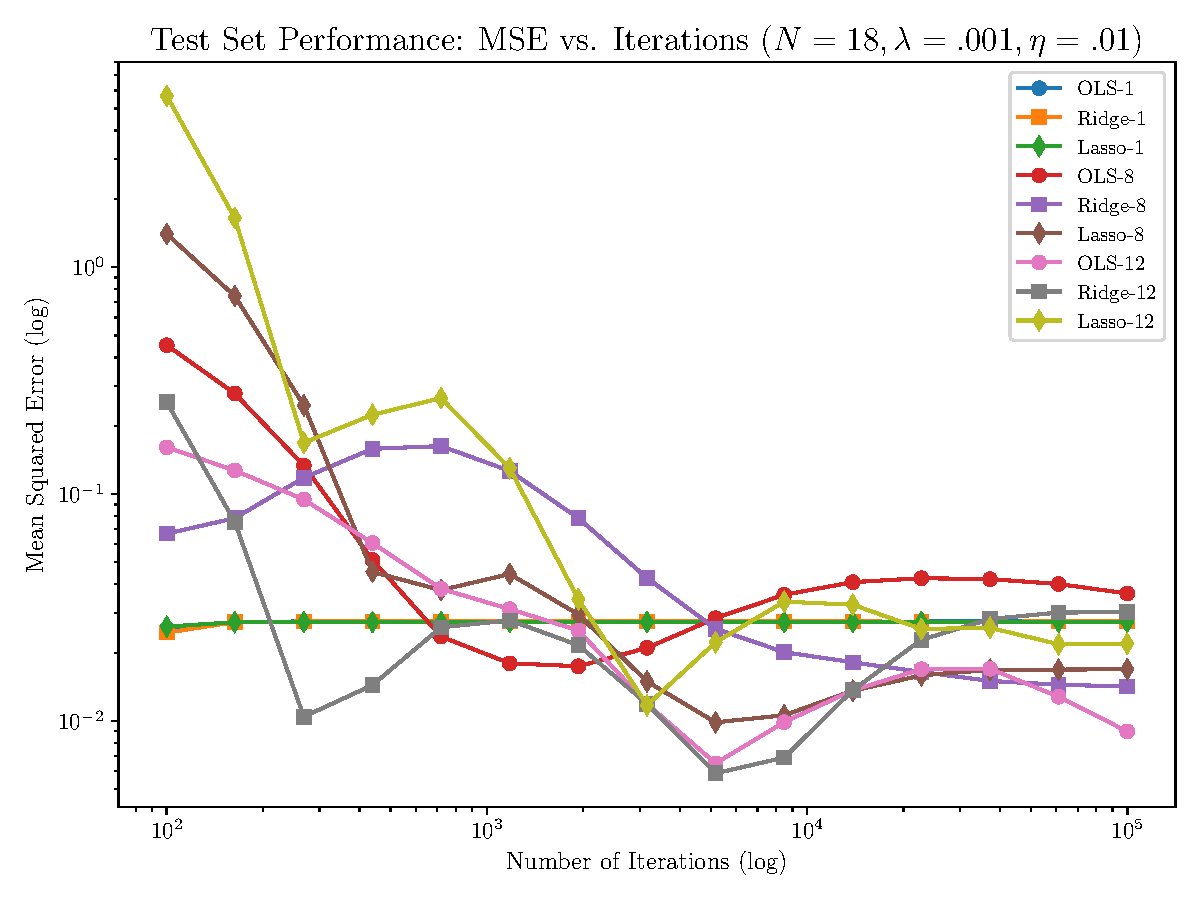
\includegraphics[width=.95 \linewidth]{Figures/StochasticDescent.pdf}
    \caption{Stochastic Gradient Descent}
    \label{fig:GradSGD}
\end{figure}
\subsection{Resampling Techniques}
Here we try to increase the performance of the model by using resampling techniques, to make the model more robust and generalizable.
In figure \ref{fig:OLS1} we see that the model is overfitting the training data and has a high variance in th more complex models.
IF we look at the test point at $x=1$ we see that the models seem to avoid it, and even the linear model has learned some bias as it has a slight tilt upwards.
Therefore we will see how the following two resampling techniques will act upon the model 


\subsubsection{Bootstrap}
Using bootstrap we do not see any improvements and instead it becomes remarkably worse on our small dataset.
This is likely due to the fact that the model is already overfitting the training data, and adding more noise through bootstrapping only exacerbates this issue.


\begin{figure}[h]
    \centering
    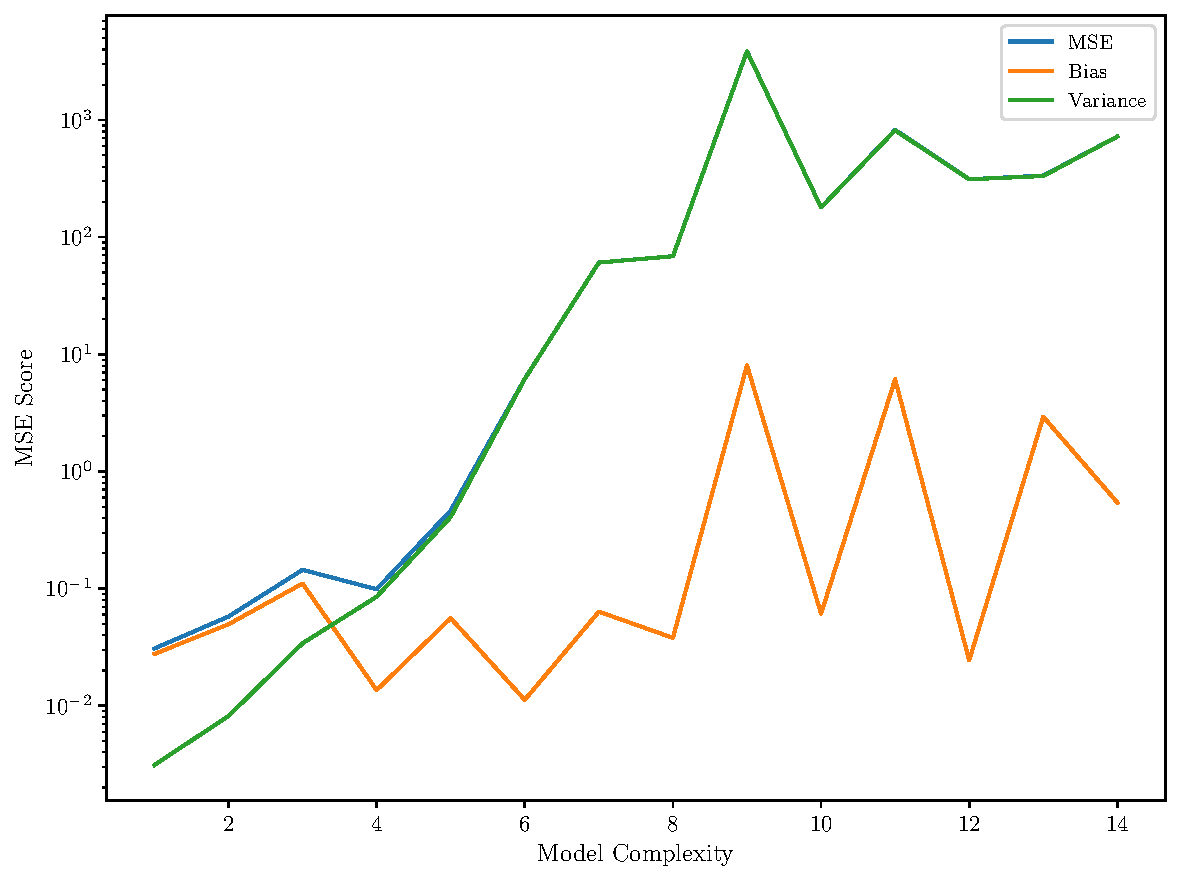
\includegraphics[width=.95 \linewidth]{Figures/Bootstrap_performance.pdf}
    \caption{Bootstrap Performance}
    \label{fig:BootstrapPerformance}
\end{figure}


\begin{figure}[h]
    \centering
    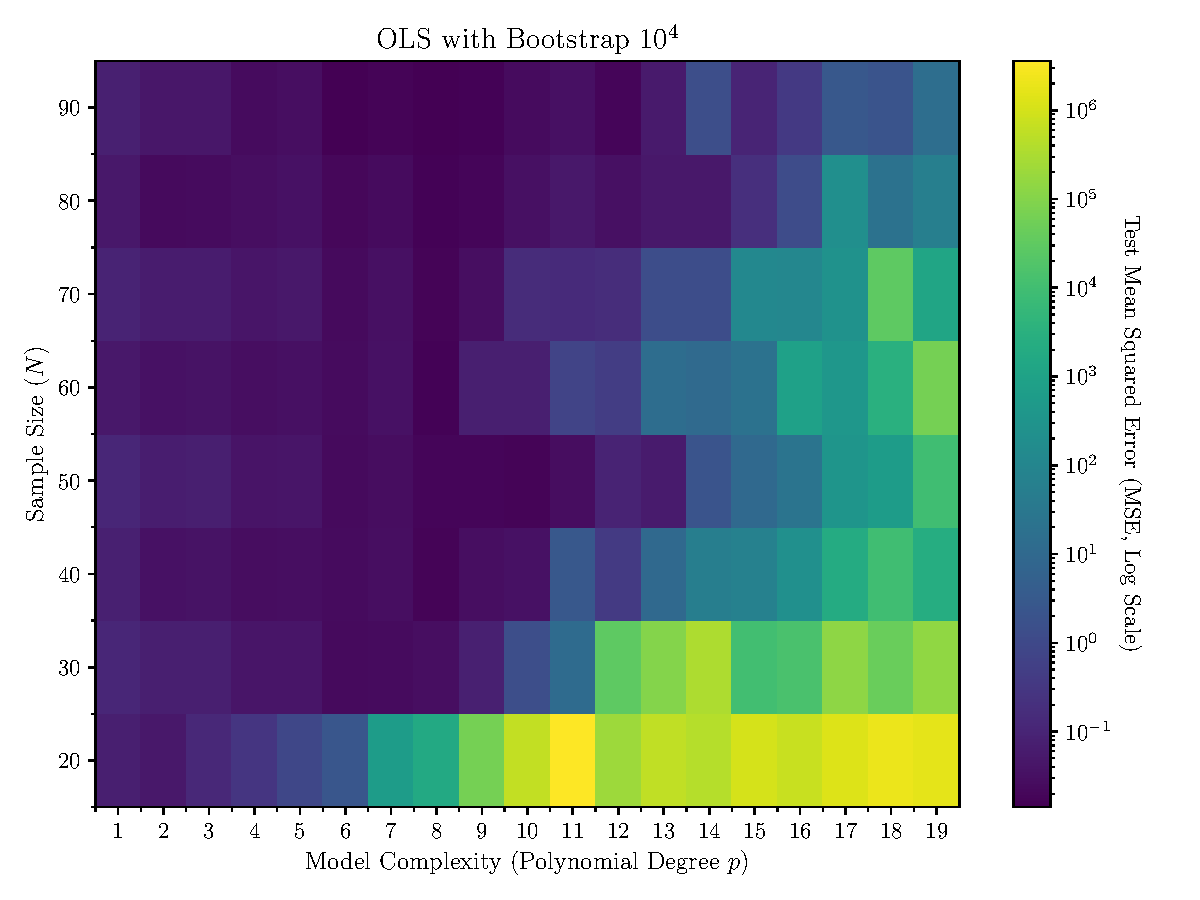
\includegraphics[width=.95 \linewidth]{Figures/Bootstrap_Heatmap.pdf}
    \caption{Bootstrap Heatmap }
    \label{fig:BootstrapHeatmap}
\end{figure}


\subsubsection{Cross Validation}
part h, k-fold cross-validation algorithm as a resampling technique on the OLS method. Compare the MSE you get from your cross-validation code with the one you got from your bootstrap code.
Comment and interpret your results.

\begin{comment}
Below you see a picture that describes the Bias-Variance trade off, \ref{fig:BiasVariance1}. 
The trade off here is visualized by having a model of higher complexity molding more and more to the training set thereby having a better fit or bias, but a worse fit on the unseen data.
Which then creates a higher variance.

When you write the results and discussion section you should focus on the following aspects:
\begin{itemize}
    \item Present your results
    \item Give a critical discussion of your work and place it in the correct context.
    \item Relate your work to other calculations/studies
    \item An eventual reader should be able to reproduce your calculations if she/he wants to do so. All input variables should be properly explained.
    \item Make sure that figures\ref{fig:BiasVariance1} and tables contain enough information in their captions, axis labels etc. so that an eventual reader can gain a good impression of your work by studying figures and tables only.
\end{itemize}


\begin{figure}[h]
    \centering
    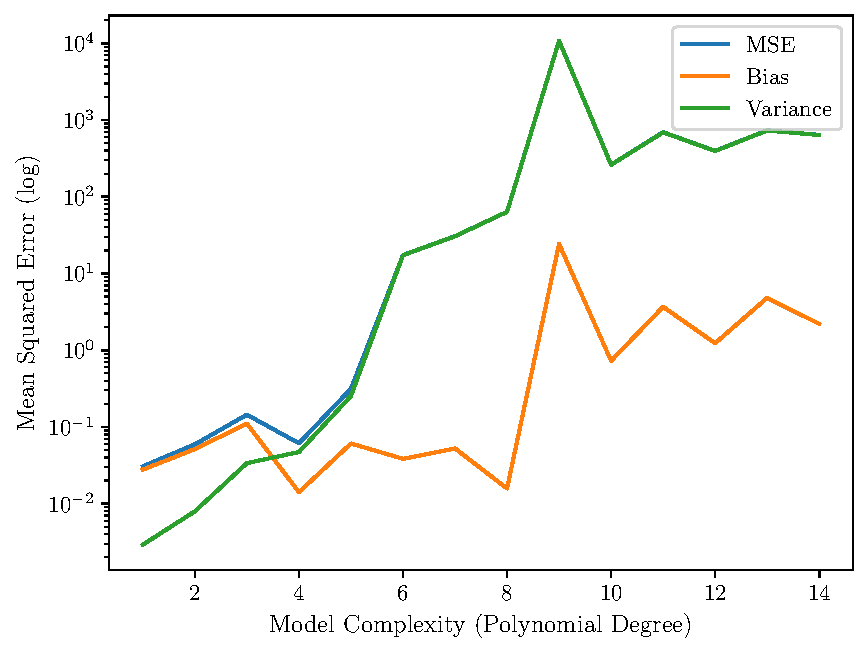
\includegraphics[width=0.9 \linewidth]{Figures/bias_variance_tradeoff.pdf}
    \caption{Bias Variance Tradeoff}
    \label{fig:BiasVariance1}
\end{figure}
Cool reference to the scikit api, \cite{sklearn_api}.


\begin{figure}[h]
    \centering
    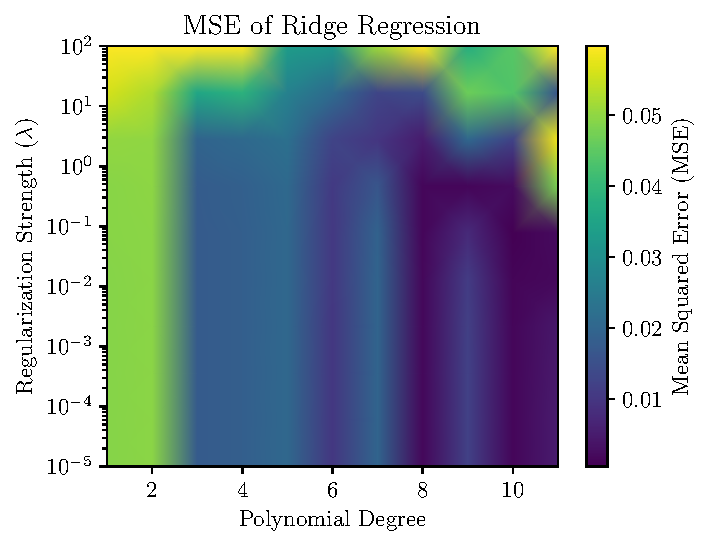
\includegraphics[width=0.9 \linewidth]{Figures/ridge_heatmap.pdf}
    \caption{Degree and Regularization Heatmap}
    \label{fig:DegRegHeat}
\end{figure}
The above heatmap, \ref{fig:DegRegHeat}, implies that a polynomial degree of 8 and a regularization value of slightly above $10^{-1} \lambda$ would be the best parameters for training the model.


\end{comment}

\section{further work}
What does striek of lines in figure \ref{fig:RidgeHeat}

\section{Conclusion}\label{section:conclusion} 
 * State your main findings and interpretations

 * Try as far as possible to present perspectives for future work

 * Try to discuss the pros and cons of the methods and possible improvements
\begin{comment}
When you write the conclusion section you should focus on the following aspects:
\begin{itemize}
    \item State your main findings and interpretations
    \item Try to discuss the pros and cons of the methods and possible improvements
    \item State limitations of the study
    \item Try as far as possible to present perspectives for future work
\end{itemize}

\end{comment}

\bibliography{biblio}



\end{document}
